\documentclass{beamer}
\graphicspath{{images/}}

\title{Intro to Git}
\date{}

\begin{document}

\frame{\titlepage}

\begin{frame}
	\frametitle{Plan}
	\begin{itemize}
		\item{Intro to Version Control}
		\item{Intro to Git}
		\item{Git Basics}
		\item{Branches in Git}
		\item{Git Reset in Detail}
	\end{itemize}
\end{frame}

\begin{frame}
	\frametitle{Intro to Version Control}
	\begin{itemize}
		\item{System that records changes to a file or set of files over time (VCS)}
		\item{Can recall specific versions at a later time}
		\item{Can revert individual files or even the entire project to a previous state}
		\item{Can compare changes in files over time}
		\item{Can see who modified something and when}
		\item{Does the very efficiently}
		\item{Set of all versions of all files called a repository}
	\end{itemize}
\end{frame}

\begin{frame}
	\frametitle{Local VCS}
	\begin{itemize}
		\item{Simple database containing all changes to file under version control}
	\end{itemize}
	\begin{figure}
		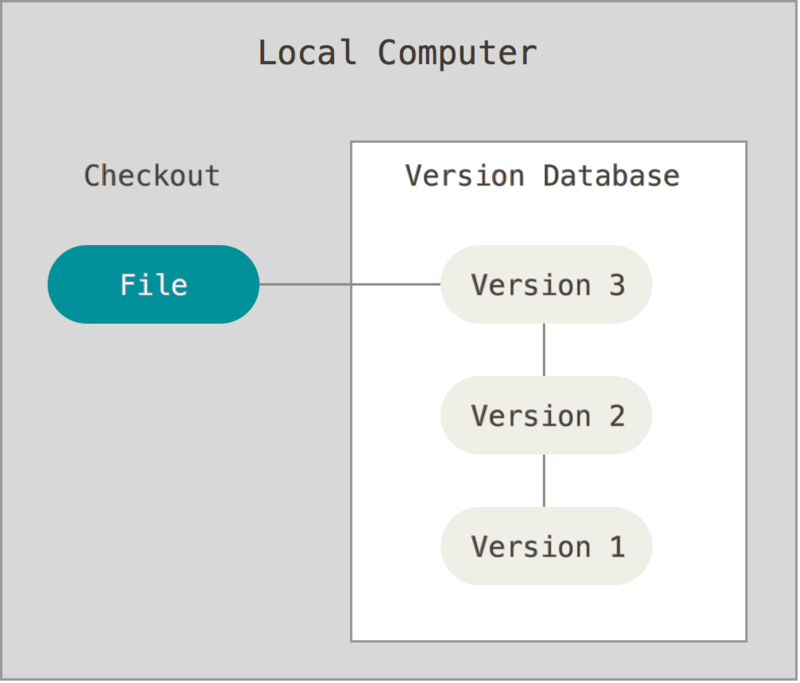
\includegraphics[scale=0.25]{Local_VCS-0.png}
	\end{figure}
\end{frame}

\begin{frame}
	\frametitle{Centralised VCS}
	\begin{itemize}
		\item{Used to collaborate with other developers}
		\item{Single server contains all the versioned files}
		\item{Clients check out snapshots from the server}
	\end{itemize}
	\begin{figure}
		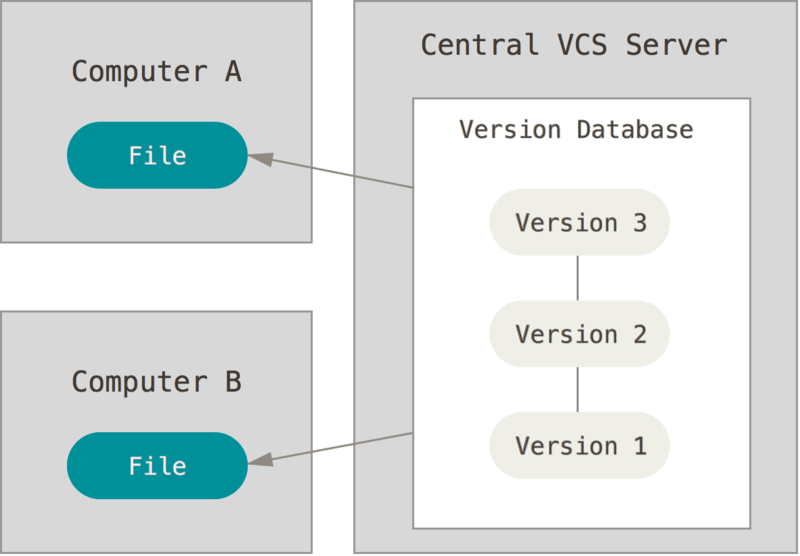
\includegraphics[scale=0.25]{Centralised_VCS-0.png}
	\end{figure}
\end{frame}

\begin{frame}
	\frametitle{Distributed VCS}
	\begin{itemize}
		\item{Each client fully mirrors the the repository}
		\item{Allows direct collaboration between developers}
	\end{itemize}
	\begin{figure}
		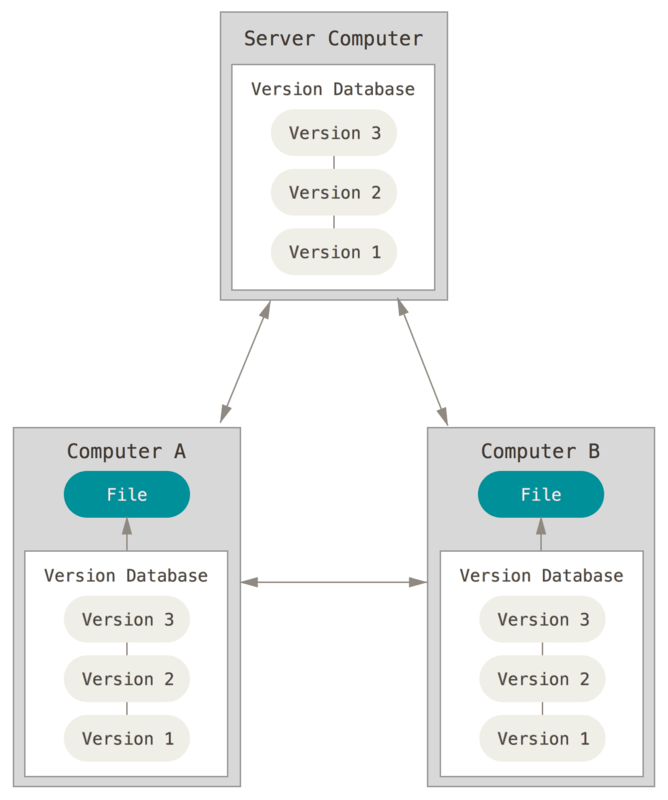
\includegraphics[scale=0.25]{Distributed_VCS-0.png}
	\end{figure}
\end{frame}

\begin{frame}
	\frametitle{A Short History of Git}
	\begin{itemize}
		\item{Created by Linus Torvalds in 2005 for Linux kernel development}
		\item{The goals for Git were:}
		\begin{itemize}
			\item{Speed}
			\item{Simple design}
			\item{Able to handle large projects}
			\item{Fully distributed}
			\item{Very good support for non-linear development}
		\end{itemize}
	\end{itemize}
\end{frame}

\end{document}

